\section{Random walk description}\label{chap:fightDef}
\begin{figure}\label{fig:randomWalk}
    \centering
    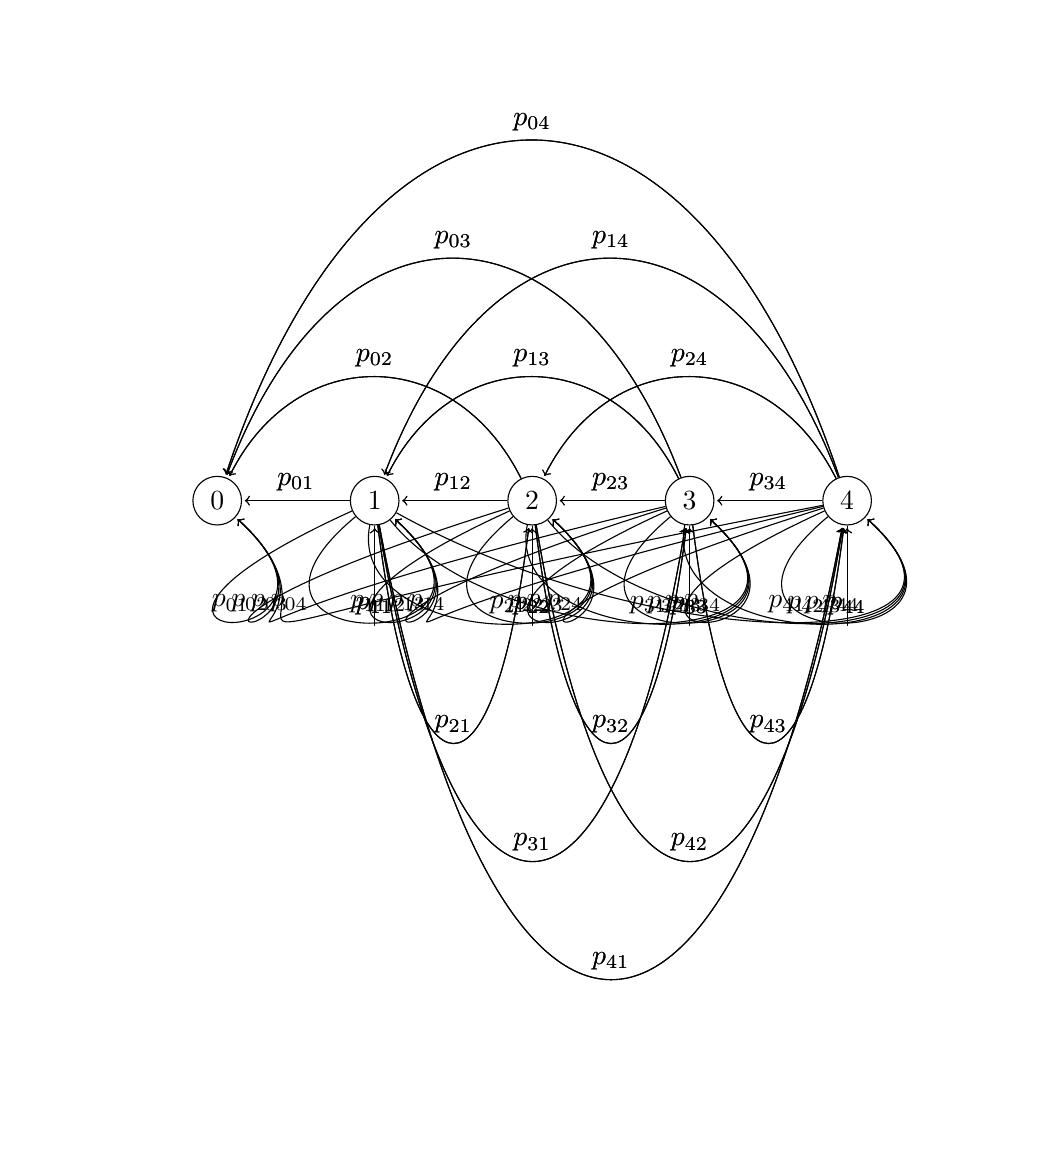
\begin{tikzpicture}[shorten >=1pt,node distance=1cm]
        \tikzstyle{state}=[shape=circle,draw,minimum size=1cm];
        \coordinate (n0);
        \xdef\scale{2}
        \xdef\maxhit{3}
        \foreach \s in {0,1,2,3,4} {
            \node[shape=circle,draw](n\s) at (\scale*\s,0){$\s$};
        }
        \foreach \from in {1,2,3,4} {
            \foreach \to in {0,1,2,3,4} {
                \foreach \y [evaluate=\y as \yeval using \from-\to] in {1} {
                \foreach \m [evaluate=\m as \meval using int(\to+\maxhit+1)] in {1} {
                    \ifthenelse{\from>\to \AND \from<\meval \AND \to>0}{
                        \path[draw,->] (n\from) ..
                        controls({(0.75*\from+0.25*\to)*\scale},{2*(\from-\to-1)}) and ({(0.25*\from+0.75*\to)*\scale},{2*(\from-\to-1)})
                        .. node[above]{$p_{\to\from}$} (n\to);
                    }{}
                    \ifthenelse{\to=0 \AND \from<\meval}{
                        \path[draw,->] (n\from) ..
                        controls({(0.75*\from+0.25*\to)*\scale},{2*(\from-\to-1)}) and ({(0.25*\from+0.75*\to)*\scale},{2*(\from-\to-1)})
                        .. node[above]{$p_{\to\from}$} (n\to);
                    }{}
                    \ifthenelse{\from=\to}{
                        \path[draw,->] (n\from) ..
                        controls({(\to-1.2)*\scale},-2) and ({(\to+1.1)*\scale},-2) .. node[above]{$p_{\to\from}$} (n\to);
                    }{}
                }
                }
            }
        }
    \end{tikzpicture}\caption{Random walk diagram for $m=3$, $h=4$ and no regeneration. The probability of walking to state $i$ from state $j$ is given with the transition probability $p_{ij}$. Only edges for which $p_{ij} > 0$ are shown.}
\end{figure}

We define the \textit{state space} as the set of all possible values remaining hitpoints can have. Every fight against an enemy with $h$ hitpoints can be thought of as a random walk in the state space $\{0,\ldots,h\}$. A walk can be labeled with a sequence of hitpoint states $(H_k)_{k=0}^{n}$ visited during the fight such that $H_0=h$ (fight starts at $h$ hitpoints), $H_n=0$ (fight ends in death) and $h \geq H_k > 0$ for $k<n$.
The probability of transitioning to state $i$ from state $j$ is called the \textit{transition probability} and is defined as
\begin{align}\label{eq:transitionProbabilities}
    p_{ij} = \Pr{H_k = i \mid H_{k-1} = j}.
\end{align}
The transition probabilities are said to have the \textit{Markov property} if they only depend on the current state. In other words, there should not be terms such as $H_{k-2}$ in the conditional probability above.

Let $\mathcal{S}_j^n$ be the set of all possible fights of length $n$ against an enemy with $j$ hitpoints remaining. The simplest case is the set of all 1-hit fights $\mathcal{S}_j^1 = \{(j,0)\}$. The sets of all longer fights can be defined recursively by noticing that if the first hit lowers the hitpoints to $i$, the remaining sequence of states is equivalent to a fight of length $n-1$ against an enemy with $i$ hitpoints remaining.
\begin{align}
    \mathcal{S}_j^n &=  \{j\} \times \bigcup_{k=1}^h \mathcal{S}_i^{n-1} \quad \mbox{for } n>1\label{eq:fightRecursion}
\end{align}
where $h$ is the maximum number of hitpoints the enemy can have. To get an idea how eq\ref{eq:fightRecursion} works consider for example the set of all 2-hit fights $\mathcal{S}_j^2 = \{(j,h,0), (j,h-1,0), \ldots, (j,2,0), (j,1,0)\}$.

Using the transition probabilities (eq\ref{eq:transitionProbabilities}) the probability that an $n$-hit fight $f \in \mathcal{S}_{j}^n$ occurs is
\begin{align}
    \Pr{f} &= \prod_{k=1}^{n} p_{f_{k} f_{k-1}}
\end{align}
where $f_k$ is the number of hitpoints the enemy has remaining after $k$ hits.

Let $L_j$ be the length of a fight against an enemy with $j$ hitpoints remaining.
By summing over all fights of length $n$ and invoking eq\ref{eq:fightRecursion} a recurrence relation for the probability that fight has length $n$ is obtained. Since the recurrence can only be applied to fights of length $2$ or higher, we treat the case $L_j = 1$ separately.
\begin{align}\label{eq:probabilityRecursion}
    \Pr{L_j = n} &= \sum_{\mathclap{f \in \mathcal{S}_j^n}}\Pr{f}
            = \sum_{i=1}^h p_{ij} \sum_{\mathclap{f \in \mathcal{S}_j^{n-1}}}\Pr{f}
            = \sum_{i=1}^h p_{ij} \Pr{L_i = n-1}\\
    \Pr{L_j = 1} &= \sum_{\mathclap{f \in \mathcal{S}_j^1}}\Pr{f}
            = \Pr{(j,0}) = p_{0j}
\end{align}
The expected length $\L_j$ of a fight can now be expressed using the definition of expectation.
\begin{align}
    \L_j = \sum_{n=1}^{\infty}n\Pr{L_j=n}
       &= \Pr{L_j=1} + \sum_{n=2}^{\infty}n\sum_{i=1}^h p_{ij} \Pr{L_i=n-1}\nonumber\\
       &= p_{0j} + \sum_{i=1}^h p_{ij} \sum_{n=2}^{\infty}n\Pr{L_i=n-1}.\label{eq:derivation2}
\end{align}
The inner sum can be worked out to be
\begin{align}
    \sum_{n=2}^{\infty}n\Pr{L_i=n-1}
       &= \sum_{n=1}^{\infty}(n+1)\Pr{L_i=n} \nonumber
       = \sum_{n=1}^{\infty}n\Pr{L_i=n} + \sum_{n=1}^{\infty}\Pr{L_i=n}
       = \L_i + 1.
\end{align}
In the last equality we used the definition of expected value as well as the fact that an enemy will be guaranteed to die if hit infinitely many times. Inserting this into eq\ref{eq:derivation2} gives
\begin{align}
    \L_j
        &= p_{0j} + \sum_{i=1}^h p_{ij}(\L_i+1)
        = \sum_{i=0}^h p_{ij} + \sum_{i=1}^h p_{ij}\L_i
\end{align}
Since the transition probabilities must add up to 1 when summed over the entire state space, we have $\sum_{i=0}^{h}p_{ij} = 1$. So the recurrence relation for the expected length of a fight can be written as
\begin{align}
    \L_j
        = 1 + \sum_{i=1}^h p_{ij}\L_i\label{eq:fightLengthRecursion}
\end{align}
